%*******************************************************%
%														%
% Steve Zekany									%
% szekany@umich.edu									%
% EECS 470 -- Lab 6										%
%														%
%*******************************************************%

%*******************************************************%
% Preamble													%
%*******************************************************%

\documentclass[table,dvipsnames]{beamer}
\usetheme{Lab}

\usepackage{
	siunitx,
	tikz,
	graphicx,
	amsmath,
	float,
	minted,
	hyperref,
	textcomp,
	upquote,
	multirow,
	fancyvrb,
	wrapfig,
	multicol
}

\usepackage[T1]{fontenc}
%-----------------------%
% TikZ					%
%-----------------------%
%--- CircuiTikZ Definitions ---%

%--- TikZ Definitions ---%
\usetikzlibrary{shapes,arrows,automata,shadows,decorations,fadings}
\pgfdeclarelayer{background}
\pgfdeclarelayer{foreground}
\pgfsetlayers{background,main,foreground}
\tikzstyle{master-blank} = 
[	draw, 
	rounded corners, 
	rectangle,
	color=ForestGreen!25,
	minimum height=0.5cm, 
	minimum width=1.30cm
]
\tikzstyle{master-commit} = 
[	draw, 
	fill=ForestGreen!50, 
	rounded corners, 
	rectangle,
	minimum height=0.5cm, 
	minimum width=1.30cm
]
\tikzstyle{branch-commit} = 
[	draw, 
	fill=RoyalBlue!70, 
	rounded corners,
	rectangle,
	minimum height=0.5cm, 
	minimum width=1.30cm
]
\tikzstyle{clean-repo} = 
[	draw, 
	inner color=RoyalBlue!40, 
	outer color=RoyalBlue!50, 
	color=black,
	circle,
	minimum height=2cm
]
\tikzstyle{changes-repo} = 
[	draw, 
	inner color=Red!40, 
	outer color=Red!50, 
	color=black,
	circle,
	minimum height=2cm
]

\definecolor{darkblue}{rgb}{0,0,0.8}

\hypersetup{colorlinks=true,linkcolor=,urlcolor=red}

\newcommand{\masterrepo}[2]{
	\scriptsize{\color{Black}\texttt{#1}} \\
	\scriptsize{\color{OliveGreen}\texttt{HEAD=#2}}
}

\newcommand{\branchrepo}[2]{
	\scriptsize{\color{Black}\texttt{#1}} \\
	\scriptsize{\color{NavyBlue}\texttt{HEAD=#2}}
}

\newcommand{\commit}[1]{
	\scriptsize{\texttt{#1}}
}

%*******************************************************%
% Document												%
%*******************************************************%

\title[Lab 6: SystemVerilog]{EECS 470 Lab 6}
\subtitle{SystemVerilog}
\institute[University of Michigan]{Department of Electrical Engineering and 
			Computer Science \\
			College of Engineering \\
			University of Michigan}
\date{Thursday, October. 10$^{\text{th}}$, 2019}

\begin{document}
\frame{\titlepage}

\begin{frame}{Overview}
	\tableofcontents
\end{frame}

\section{Administrivia}
\begin{frame}{Crazy times are here}
	\begin{block}{Project}
		\begin{itemize}
			\item Milestone 1 is due Wednesday, October 23$^{\text{rd}}$!
			\begin{itemize}
				\item You should have at least one module fully completed and debugged
				\item Turn in: progress report, and one module and testbench for us to grade
				\item Some resources (like fast priority selector) are available on the \href{http://www.eecs.umich.edu/courses/eecs470/?page=project.php}{course site}!
			\end{itemize}
		\end{itemize}
	\end{block}
\end{frame}

\section{Motivation}
\begin{frame}{Motivation}
	\begin{block}{Why SystemVerilog? Why now?}
		\begin{itemize}
			\item Extra features that will be useful in your projects
			\item Not all features are easy to use: many have a steep learning curve
			\item The goal isn't to go wild and try to use everything...
			\item Instead, think about which are worthwhile to incorporate
		\end{itemize}
	\end{block}
\end{frame}

\begin{frame}{What is SystemVerilog?}
	\begin{block}{}
		\begin{enumerate}
			\item 1995 -- Verilog HDL
			\item 2001 -- Verilog 2001 
			\item 2005 -- SystemVerilog
		\end{enumerate}
		\begin{itemize}
			\item Emphasis on creating a combined Hardware Description Language and Hardware Verification Language
			\item Ability to debug at the ``system'' level
			\item Provides the basis for very powerful, object-oriented testbenches
			\item The framework for industry verification tools, e.g. UVM
		\end{itemize}

	\end{block}
\end{frame}


\section{Multidimensional Arrays}
\begin{frame}{Multidimensional Arrays}
	\begin{block}{Example}
		\begin{itemize}
			\item \texttt {logic [127:0] [63:0] multi\_d\_array [3:0];}
			\item \texttt {assign multi\_d\_array[3][101] = 64'hFFFF\_FFFF;}
		\end{itemize}
	\end{block}
	\begin{block}{Explanation}
		\begin{itemize}
			\item ``[127:0]'' and ``[63:0]'' are called ``packed'' dimensions
			\item ``[3:0]'' is an ``unpacked'' dimension 
			\item When referencing for read/write, unpacked dimensions come first, then packed dimensions
		\end{itemize}
	\end{block}
\end{frame}

\begin{frame}{Multidimensional Arrays}
	\begin{block}{Example}
		\begin{itemize}
			\item \texttt {logic [127:0] [63:0] multi\_d\_array [3:0];}
			\item \texttt {assign multi\_d\_array[3][101] = 64'hFFFF\_FFFF;}
		\end{itemize}
	\end{block}
	\begin{block}{Explanation}
		\begin{itemize}
			\item Old Verilog only allows one packed dimension 
			\item SystemVerilog allows as many as you need 
			\item We recommend packed arrays for most designs
			
		\end{itemize}
	\end{block}
\end{frame}

\begin{frame}{Multidimensional Arrays}
	\begin{block}{Example}
		\begin{itemize}
			\item \texttt {logic [31:0] one\_d\_array;}
			\item \texttt {logic [15:0] [1:0] two\_d\_array;}
			\item \texttt {assign two\_d\_array = one\_d\_array;}
		\end{itemize}
	\end{block}
	\begin{block}{Explanation}
		\begin{itemize}
			\item Packed arrays are laid out as a contiguous set of bits
			\item Allows easy copying from one array to another
		\end{itemize}
	\end{block}
\end{frame}
 
 \section{Unique and Priority}
 \begin{frame}[fragile]{Unique/priority if/case}
	\begin{minted}{verilog}
input a, b, c;
input [1:0] sel;
output z;
case (sel)
	2'b00: z = a;
	2'b01: z = b;
	2'b10: z = c;
endcase	
	\end{minted}
	\begin{block}{}
		How will the synthesis tool convert this design to hardware?
	\end{block}

\end{frame}
 
 
\begin{frame}[fragile]{Unique/priority if/case}
		\begin{wrapfigure}{r}{0.55\textwidth}
			\centering
			 %\vspace{-160pt} % This removes the white box on the second page
			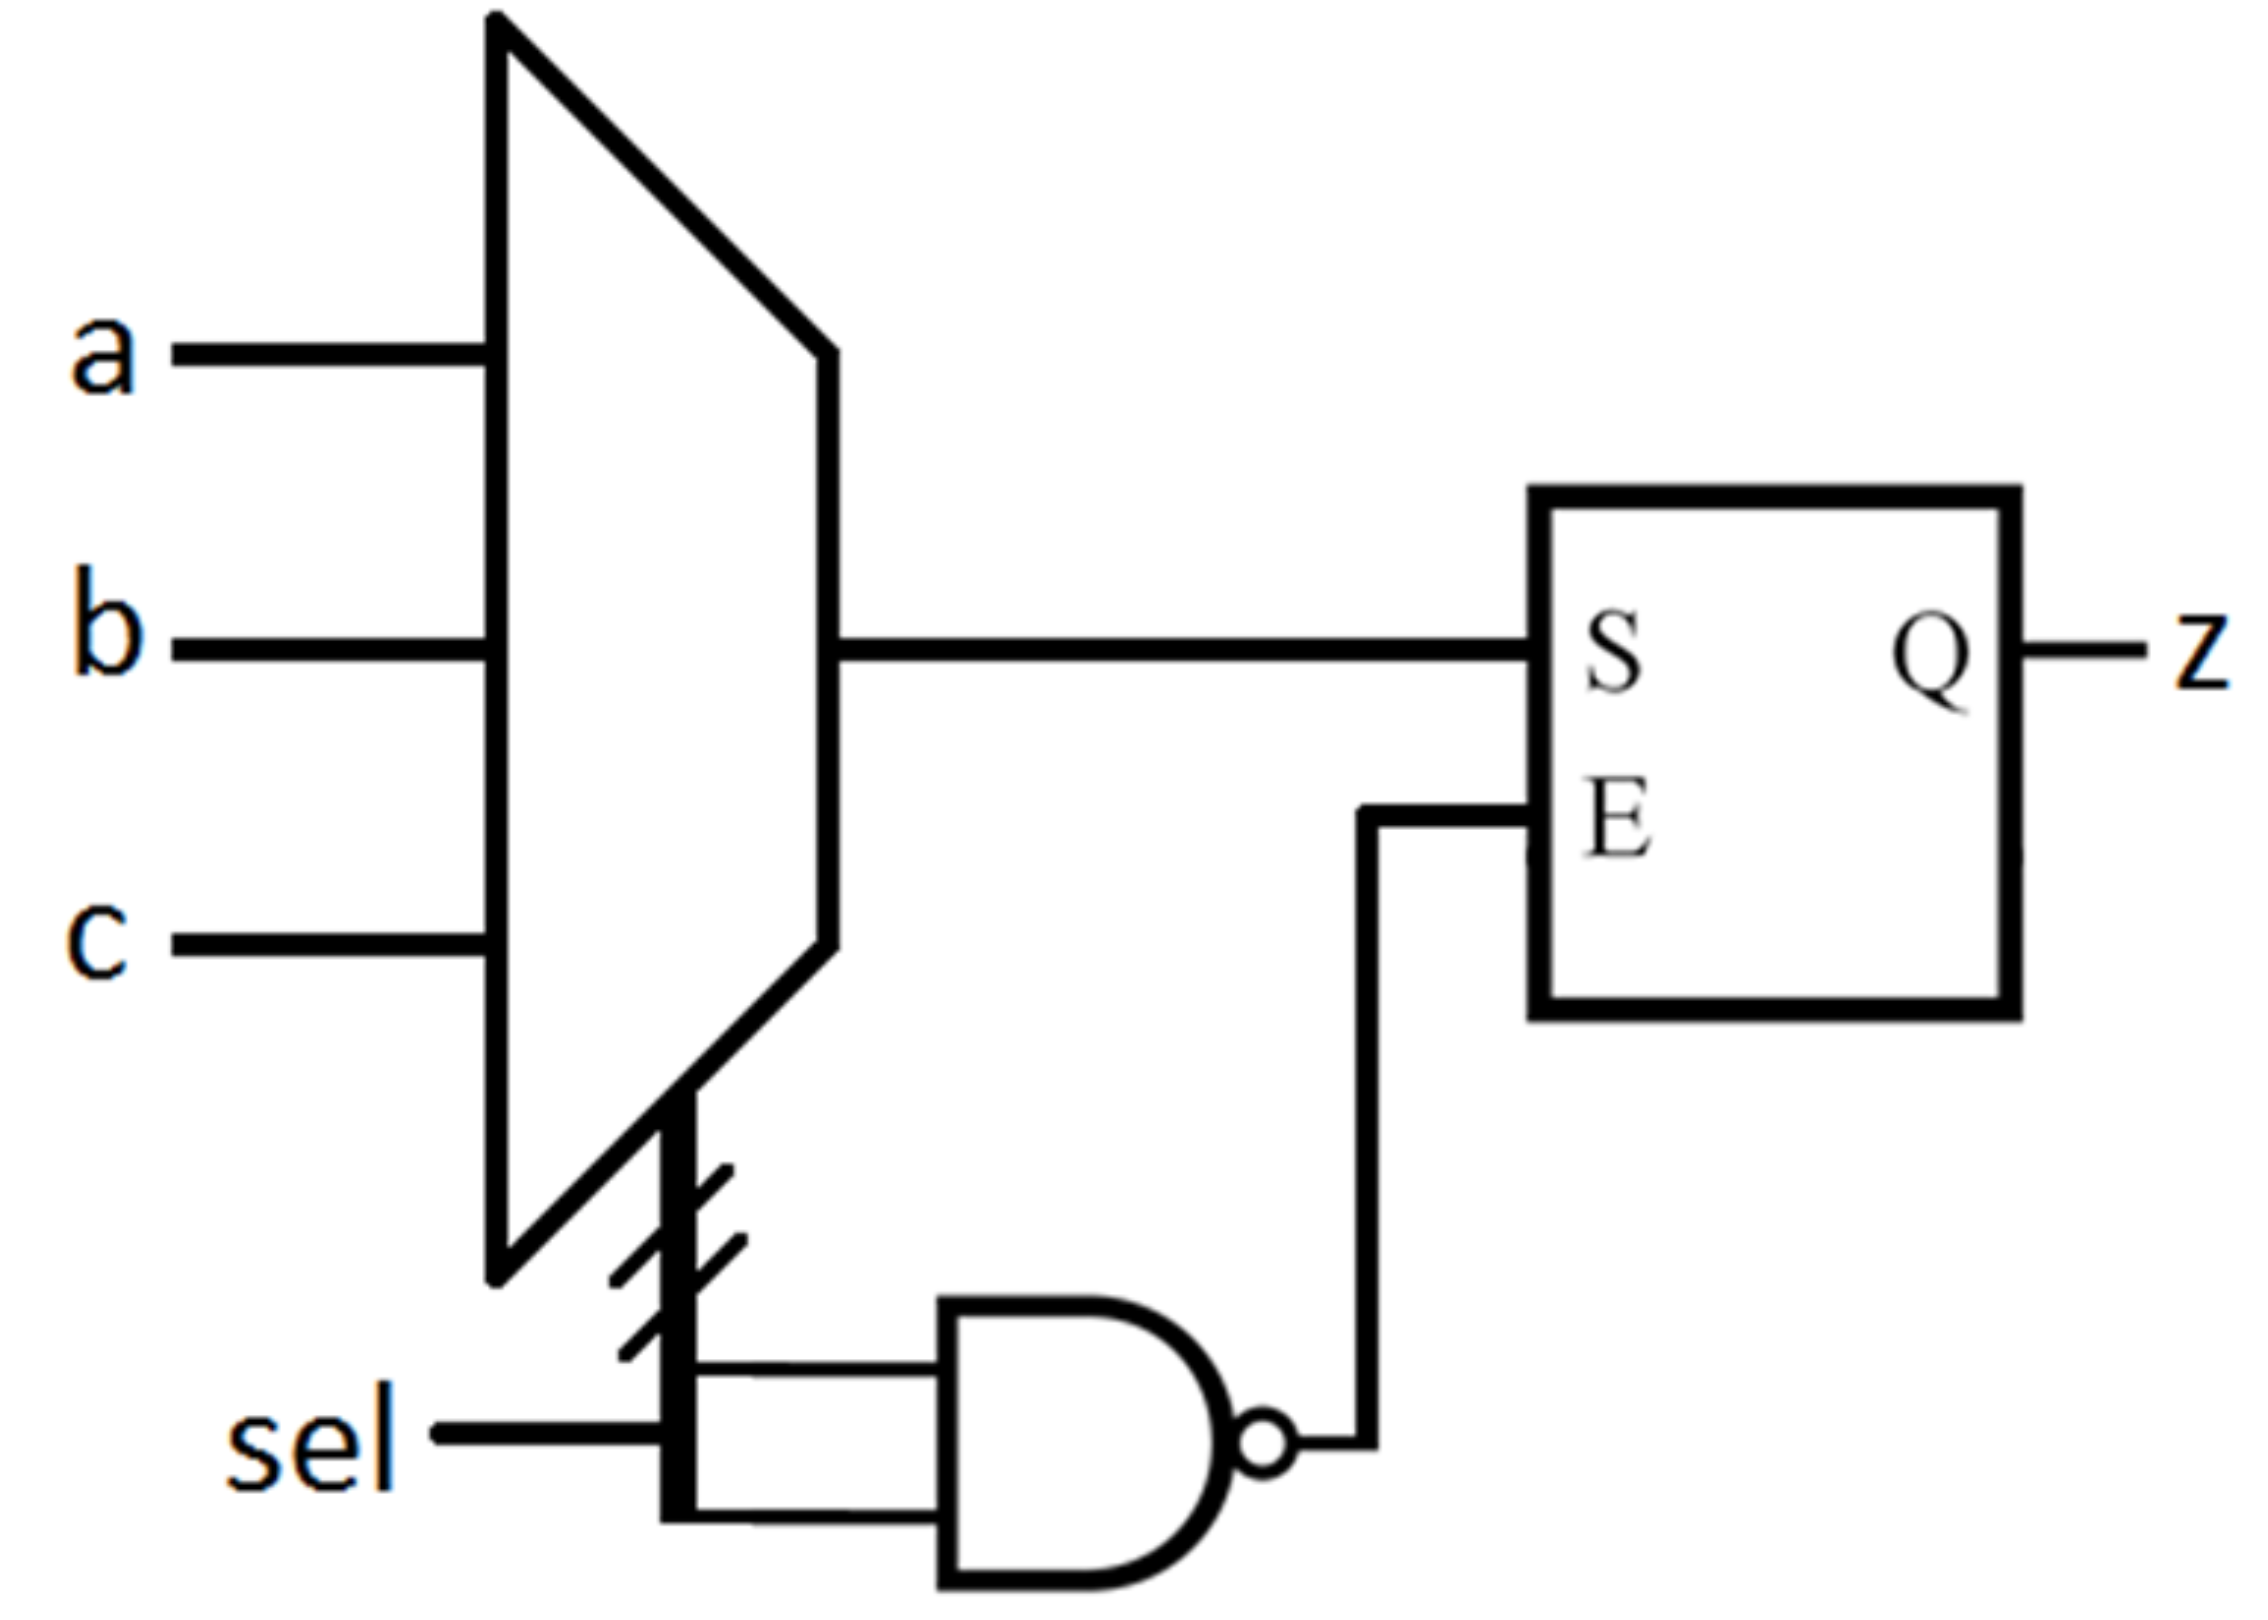
\includegraphics[width=\textwidth]{latch.png}
		\end{wrapfigure}

	\begin{minted}{verilog}
input a, b, c;
input [1:0] sel;
output z;
case (sel)
	2'b00: z = a;
	2'b01: z = b;
	2'b10: z = c;
endcase	
	\end{minted}
	\begin{block}{}
		A latch will be generated, since a value for z was not specified when 
		\newline sel == 2'b11
	\end{block}

\end{frame}
 
 
 
  \begin{frame}{Unique/priority if/case}
	\begin{block}{What if you know sel will never equal 2'b11?}
		\begin{itemize}
			\item You could add a dummy state, but that adds unnecessary logic and potentially hides errors
			\item SystemVerilog has a ``priority'' construct for exactly this problem
			\begin{itemize}
				\item Tells synthesis tool not to generate a latch
				\item Checks at run-time that each state is reachable
			\end{itemize}
		\end{itemize}
	\end{block}
\end{frame}


 
  \begin{frame}[fragile]{Unique/priority if/case}
	\begin{minted}{verilog}
input a, b, c;
input [1:0] sel;
output z;
priority case (sel)
	2'b00: z = a;
	2'b01: z = b;
	2'b10: z = c;
endcase
	\end{minted}
	\begin{block}{}
		During behavioral simulation, if sel is 2'b11, a warning will be generated:
		\\\\\color{red} RT Warning: No condition matches in priority case statement.
	\end{block}

\end{frame}
 
 
  \begin{frame}[fragile]{Unique/priority if/case}
  \begin{block}{Another code example:}
	\begin{minted}{verilog}
input [1:0] sel;
output logic [1:0] z;
if (sel[1])
	z = a;
else if (sel[0])
	z = b;
else
	z = c	
	\end{minted}
	\end{block}
	\begin{block}{What hardware will be generated by this code?}
	\end{block}

\end{frame}
 
 
 
 
   \begin{frame}[fragile]{Unique/priority if/case}
   	\begin{wrapfigure}[0]{r}{0.6\textwidth}
			\centering
			%\vspace{-100pt}
			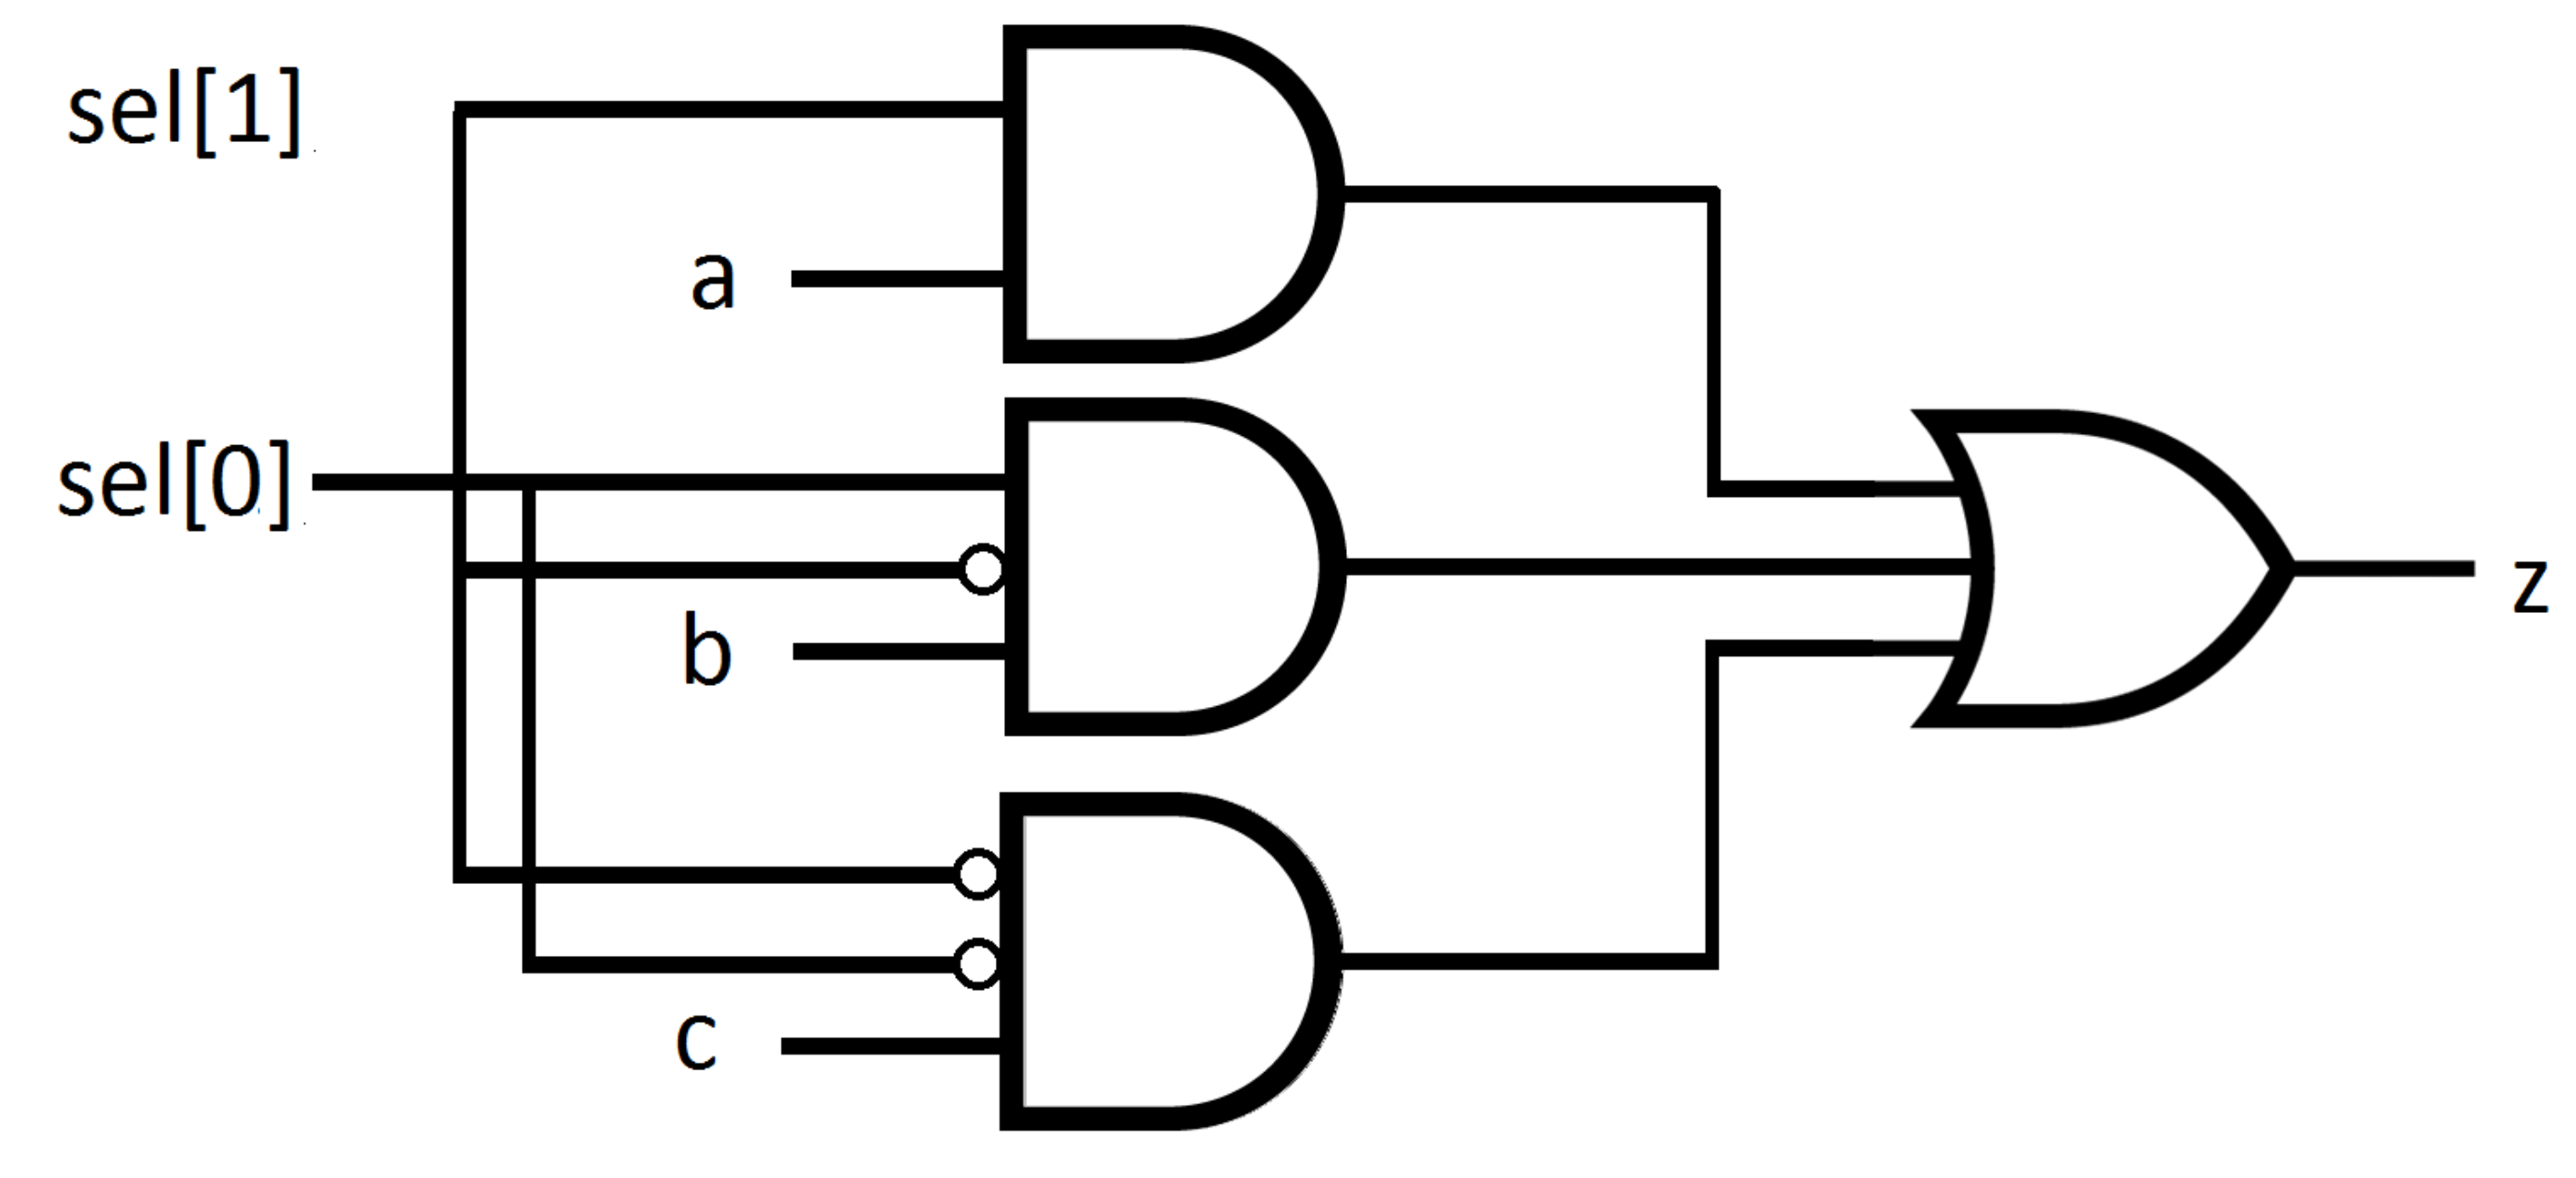
\includegraphics[width=\textwidth]{multiple_bits.png}
	\end{wrapfigure}
	

  \begin{block}{Another code example:}
	\begin{minted}{verilog}
input [1:0] sel;
output logic [1:0] z;
if (sel[1])
	z = a;
else if (sel[0])
	z = b;
else
	z = c	
	\end{minted}
	\end{block}
	\begin{block}{Tool will give priority to higher bits, since it assumes multiple bits could be high?}
		\begin{itemize}
			\item But what if we're using one-hot encoding?
		\end{itemize}
	\end{block}
\end{frame}
 
 
 
  
  \begin{frame}[fragile]{Unique/priority if/case}
  \begin{multicols}{2}
  [\begin{block}{SystemVerilog has ``unique'' if/case statement} \end{block}]
  \begin{block}{}
	\begin{minted}{verilog}
input [1:0] sel;
output logic [1:0] z;
unique if (sel[1])
	z = a;
else if (sel[0])
	z = b;
else
	z = c	
	\end{minted}
	\end{block}
	\begin{block}{}
	\begin{itemize}
		\item Tells synthesis tool to assume \\ one-hot encoding
		\item Ignores priority logic and doesn't \\ generate any latches
		\item Generates simulation warning \\ if multiple bits are high
	\end{itemize}
	\end{block}
	\end{multicols}
\end{frame}
 
   \begin{frame}{Unique/priority if/case}
	\begin{block}{Unique \& Priority used for both if and case statements}
		\begin{itemize}
			\item Replaces ``full\_case'' and ``parallel\_case'' pragmas from old Verilog
			\item Useful for simplifying logic and clarifying design choices
		\end{itemize}
	\end{block}
\end{frame}

 \section{Assertions}
   \begin{frame}{Assertions}
	\begin{block}{Assertions}
		\begin{itemize}
			\item Strategy for automated testing: check that certain conditions are true
			\item Statements declaring some kind of invariant
			\item Can be inserted in testbenches or RTL (ignored by synthesis)
			\item Two types:
			\begin{itemize}
				\item Immediate: directly called in code
				\item Concurrent: running in background
			\end{itemize}
		\end{itemize}
	\end{block}
\end{frame}

\begin{frame}[fragile]{Immediate Assertions}
	\begin{block}{Need to check that some expression is true...}
			\begin{minted}{verilog}
adder a1(a, b, c);
initial begin
	if ((a+b) != c)
	$display("Error!");
end
		\end{minted}
	\end{block}
	\begin{block}{Better done by immediate assertion...}
		\begin{minted}{verilog}
adder a1(a, b, c);
initial begin
	assert ((a+b) == c);	
end
		\end{minted}
	\end{block}
\end{frame}

 
    \begin{frame}{Concurrent Assertions}
	\begin{block}{}
		\begin{itemize}
			\item Much more interesting (and challenging)
			\begin{itemize}
				\item Describe high-level functional correctness of your design...
				\item ...and have simulator check these invariants in the background
			\end{itemize}
			\item SystemVerilog supports an entire assertion language (!)
			\begin{itemize}
				\item (beyond the scope of what we will do in class)
			\end{itemize}
			\item Implication 
			\begin{itemize}
				\item \color{ForestGreen} \texttt{s1 |-> s2}
				\begin{itemize}
					\item \color{Black} If s1 is true, then s2 must also be true
				\end{itemize}
			\end{itemize}
			\item Timing windows
			\begin{itemize}
				\item \color{ForestGreen} \texttt{(a \&\& b) |-> \#\#[1:3] c;}
				\begin{itemize} 
					\item \color{Black} On the posedge of the clock, if a and b are true, then 1-3 cycles later, c will be true
				\end{itemize}
			\end{itemize}

			
		\end{itemize}
	\end{block}
\end{frame}
 
 
    \begin{frame}{Assertions}
	\begin{block}{Assertions}
		\begin{itemize}
			\item For more information on assertions, check out ``\href{https://mirlyn.lib.umich.edu/Record/005702668}{A Practical Guide to SystemVerilog Assertions}''
		\end{itemize}
	\end{block}
\end{frame}

 \section{For Loops}
 \begin{frame}[fragile]{``For'' loops}
	\begin{block}{\textit{``You want `for' loops? You can't handle `for' loops!''}}
		\begin{itemize}
			\item We told you earlier in the semester that ``for'' loops are not a thing
			\item We lied, sort of... but they don't work the way they do in software
			\item In software we think about iterations of loops
			\begin{itemize} 
				\item Iteration 1, then Iteration 2, then Iteration 3... etc...
			\end{itemize}
			\item In hardware, loops need to unroll completely at design time
			\begin{itemize}
				\item Self-modifying hardware is still not a thing...
				\item So either everything runs in parallel (good)
				\item Or loop can ``break'' when a certain condition is true (can get ugly)
			\end{itemize}
		\end{itemize}
	\end{block}
\end{frame}
 
 
 
     \begin{frame}[fragile]{For loops}
	\begin{block}{Does this make sense for actual hardware?}
		\begin{itemize}
			 \begin{minted}{verilog}
parity = 0;
for (int i=0; i<32; i++) begin
 	if (in[i])
		parity = ~parity;
end			
\end{minted}
			
		\end{itemize}
	\end{block}
\end{frame}

 
     \begin{frame}[fragile]{For loops}
	\begin{block}{Designing synthesizable ``for'' loops}
		\begin{itemize}
			\item ``For'' loops can be valuable, just different than software
			\begin{itemize}
				\item Just another way of doing combinational logic, not a replacement for sequential logic
				\item Very limited ability to change signals referenced in the loop
			\end{itemize}
			\item Great for condensing repetitive code, because everything will be done in parallel
			\item Visualize how a loop can be built into hardware at synthesis time 
			%\item Watch out for circular logic!

		\end{itemize}
	\end{block}
\end{frame}



     \begin{frame}[fragile]{For loops}
	\begin{block}{Blocking assignment in loops}
		\begin{itemize}
			 \begin{minted}{verilog}
always_comb begin
	for (int i=0; i<32; i++)
		a = i;
end
			\end{minted}
			\item What will a equal?
			\item 31, because if we unrolled the loop, the assignment to 31 would be last
		\end{itemize}
	\end{block}
\end{frame}



     \begin{frame}[fragile]{For loops}
	\begin{block}{Break Statements}
		\begin{itemize}
			 \begin{minted}{verilog}
always_comb begin
	for (int i=0; i<32; i++)
		a = i;
		if (condition[i]) break;
end
			\end{minted}
			\item Effect: break out of loop once condition is true
			%\item Break statements are synthesizable, but be cautious: lots of hidden priority logic is required behind the scenes to make this work
			%\item You will typically get better performance by building in a different (better) way
					\end{itemize}
	\end{block}
\end{frame}

\begin{frame}[fragile]{For loops}
	\begin{block}{Max loop iterations}
			\begin{itemize}
			 	\item Design Compiler sets a maximum number of loop iterations to prevent infinite loops
			 	\begin{itemize}
			 		\item This is configured to be 1024 by default
			 		\item If you need more, add this line to your .tcl file:
			 		\\\texttt{set hdlin\_while\_loop\_iterations (iterations)}
				\end{itemize}
			\end{itemize}
	\end{block}


	\begin{block}{Final advice}
		\begin{itemize}
			 \item Remember: don't use Verilog as a way to avoid thinking about actual hardware
			 \begin{itemize}
			 	\item This results in synthesis problems or overly complex designs
			\end{itemize}
			\item First think about how to build the hardware, then think about the Verilog constructs that can allow you to describe your design easily
			\end{itemize}
	\end{block}
\end{frame}
 
 
  \section{Generate Blocks}
    \begin{frame}[fragile]{Generic Designs}
	\begin{block}{Goal: complex designs with a single parameter}
		\begin{itemize}
			\item Want to make designs where we can easily change certain features
			\begin{itemize}
				\item For example, the number of ROB entries
			\end{itemize}
			\item The multiplier in P2 could be modified using parameters
			\item We can build complex designs... remember module arrays?
			 \begin{minted}{verilog}
one_bit_adder add_8 [7:0] (
	.a(a), .b(b), .cin({carries, cin}), 
	.sum(sum), .cout({cout, carries}));
			\end{minted}
			
			
			\item \color{Black} What if we couldn't condense everything to a single parameter?
			\begin{itemize}
				\item An adder is simple, just an array of smaller adders
				\item What about more complex structures like the priority selectors from P1 that are trees of smaller selectors?
			\end{itemize}
		\end{itemize}
	\end{block}
\end{frame}
 

     \begin{frame}[fragile]{Generate Blocks}
	\begin{block}{Generate blocks give control}
		\begin{itemize}
			\item Using a generate block to build hardware:
			\begin{minted}[tabsize=4]{verilog}
generate
	genvar i;
	for (i=0; i<N; i++) begin
		one_bit_adder (
			.a(a[i]), .b(b[i]), 
			.cin(carries[i]), 
			.sum(sum[i]), 
			.cout(carries[i+1]));
	end
endgenerate
			\end{minted}
			\end{itemize}
	\end{block}
\end{frame}
 
 
     \begin{frame}[fragile]{Generic Designs}
	\begin{block}{Goal: complex designs with a single parameter}
		\begin{itemize}
			\item How does this work?
			\begin{itemize}
				\item The tool will ``elaborate'' the design
				\item Evaluate ``if'' statements and unroll ``for'' loops
			\end{itemize}
			\item Important: all conditions must be deterministic at compile time
		\end{itemize}
	\end{block}
\end{frame}
 
\begin{frame}[fragile]{Generate Blocks}
	\begin{block}{Another example: the Priority selectors from P1:}
		 \begin{minted}[tabsize=4]{verilog}
generate
	genvar i;
	for (i=0; i<N; i++) begin
		localparam left_right = i[0];
		
		ps2 (
			.req		(sub_reqs[i]),
			.en 		(sub_gnts[i/2][left_right])
			.gnt		(sub_gnts[i]),
			.req_up	(sub_reqs[i/2][left_right]))
	end
endgenerate
			\end{minted}
	\end{block}
\end{frame}
 
 
 


 
 
 

\section{Assignment}
\begin{frame}[fragile]{Lab Assignment}
	\begin{itemize}
		\item Assignment is posted to the course website as 
			\href{http://www.eecs.umich.edu/courses/eecs470/labs/eecs470lab6assignment.pdf}{Lab
			6 Assignment}.
		\item If you get stuck\dots
			\begin{itemize}
				\item Ask a neighbor, quietly
				\item Put yourself in the 
					\href{https://oh.eecs.umich.edu/courses/eecs470}{help queue}
			\end{itemize}
		\item When you finish the assignment, sign up in the
			\href{https://oh.eecs.umich.edu/courses/eecs470}{help queue}
			and mark that you would like to be checked off.
		\item If you are unable to finish today, the assignment needs to be
			checked off by a GSI in office hours \emph{before} the end of next week.
	\end{itemize}
\end{frame}

\end{document}
